\documentclass[12pt,a4paper,onecolumn]{exam}

\usepackage{amsmath}
\usepackage{amsthm}
\usepackage{amssymb}
\usepackage{graphicx}
\usepackage{float}
\usepackage[top=1in, bottom=1in, left=0.75in, right=0.75in]{geometry}
\usepackage{tikz}
\usepackage[skins]{tcolorbox}
\usepackage{listings}
\usepackage{xcolor}
\usepackage{hyperref}
\usepackage{multirow}
\usepackage{adjustbox}
\usepackage{booktabs}
\usepackage[font=small]{caption}
\usepackage{subcaption}

% --- Code Listing Colors ---
\definecolor{codegreen}{rgb}{0,0.6,0}
\definecolor{codegray}{rgb}{0.5,0.5,0.5}
\definecolor{codepurple}{rgb}{0.58,0,0.82}
\definecolor{backcolour}{rgb}{0.95,0.95,0.92}

% --- Code Listing Style ---
\lstdefinestyle{mystyle}{
    backgroundcolor=\color{backcolour},
    commentstyle=\color{codegreen},
    keywordstyle=\color{magenta},
    numberstyle=\tiny\color{codegray},
    stringstyle=\color{codepurple},
    basicstyle=\ttfamily\footnotesize,
    breaklines=true,
    captionpos=b,
    keepspaces=true,
    numbers=left,
    numbersep=2pt,
    showspaces=false,
    showstringspaces=false,
    showtabs=false,
    tabsize=1
}

\newcommand{\questionheader}[1]{%
  \begin{tcolorbox}[
    enhanced,
    colback=black,
    coltext=white,
    boxrule=0pt,
    fontupper=\Large\bfseries,
    arc=4mm
  ]
  #1
  \end{tcolorbox}%
}

\lstset{style=mystyle, language=Python}
\pagestyle{headandfoot}
\runningheader{Assignment 3}{Advanced Image Processing}{Dwaipayan Haldar}

\begin{document}

\begingroup
    \centering
    \LARGE E9 246 Advanced Image Processing\\
    \LARGE Assignment 3\\[0.5em]
    \large Dwaipayan Haldar\par
    \large \today\\[0.5em]
\endgroup
\noindent\rule{\textwidth}{0.5pt}
\printanswers
\renewcommand{\solutiontitle}{\noindent\textbf{Ans:}\enspace}

%----------------------------------------------------------------------
\questionheader{Problem 1: Block Matching and 3D Filtering}
%----------------------------------------------------------------------

\textbf{Subpart 1}
\begin{solution}

BM3D denoising proceeds in two stages. In \textbf{Stage~1}, similar 2-D patches are grouped into 3-D arrays by block matching, a 3-D transform is applied, and hard thresholding (HT) is performed with threshold $\lambda_{\mathrm{3D}}\,\sigma$ to produce the basic estimate $\hat{y}^{\mathrm{ht}}$. In \textbf{Stage~2}, the same grouping procedure is repeated, but a Wiener filter is applied in the transform domain using $\hat{y}^{\mathrm{ht}}$ as the pilot signal-spectrum estimate:
\[
  w_m = \frac{|\hat{Y}^{\mathrm{ht}}_m|^2}{|\hat{Y}^{\mathrm{ht}}_m|^2 + \sigma^2},
\]
where $\hat{Y}^{\mathrm{ht}}_m$ is the $m$-th 3-D transform coefficient of the basic estimate. This yields the final estimate $\hat{y}^{\mathrm{wie}}$.

The noisy cameraman image ($\sigma = 0.2$, images normalised to $[0,1]$) was denoised with both stages. MSE values with respect to the clean image are reported below.

\begin{center}
\begin{tabular}{lc}
\toprule
Estimate & MSE \\
\midrule
Noisy input & 0.02580 \\
Stage 1 --- HT only & 0.00994 \\
Stage 2 --- HT $+$ Wiener & 0.00709 \\
\bottomrule
\end{tabular}
\end{center}

Stage 2 achieves a 28.7\% reduction in MSE compared to Stage 1. This is expected: the Wiener filter is the linear minimum mean-square-error (LMMSE) estimator given the noise PSD and the signal spectrum, whereas HT uses a single fixed threshold regardless of the true signal amplitude. Wiener shrinkage is therefore adaptive and signal-aware, preserving large-coefficient details more faithfully.

\begin{figure}[H]
  \centering
  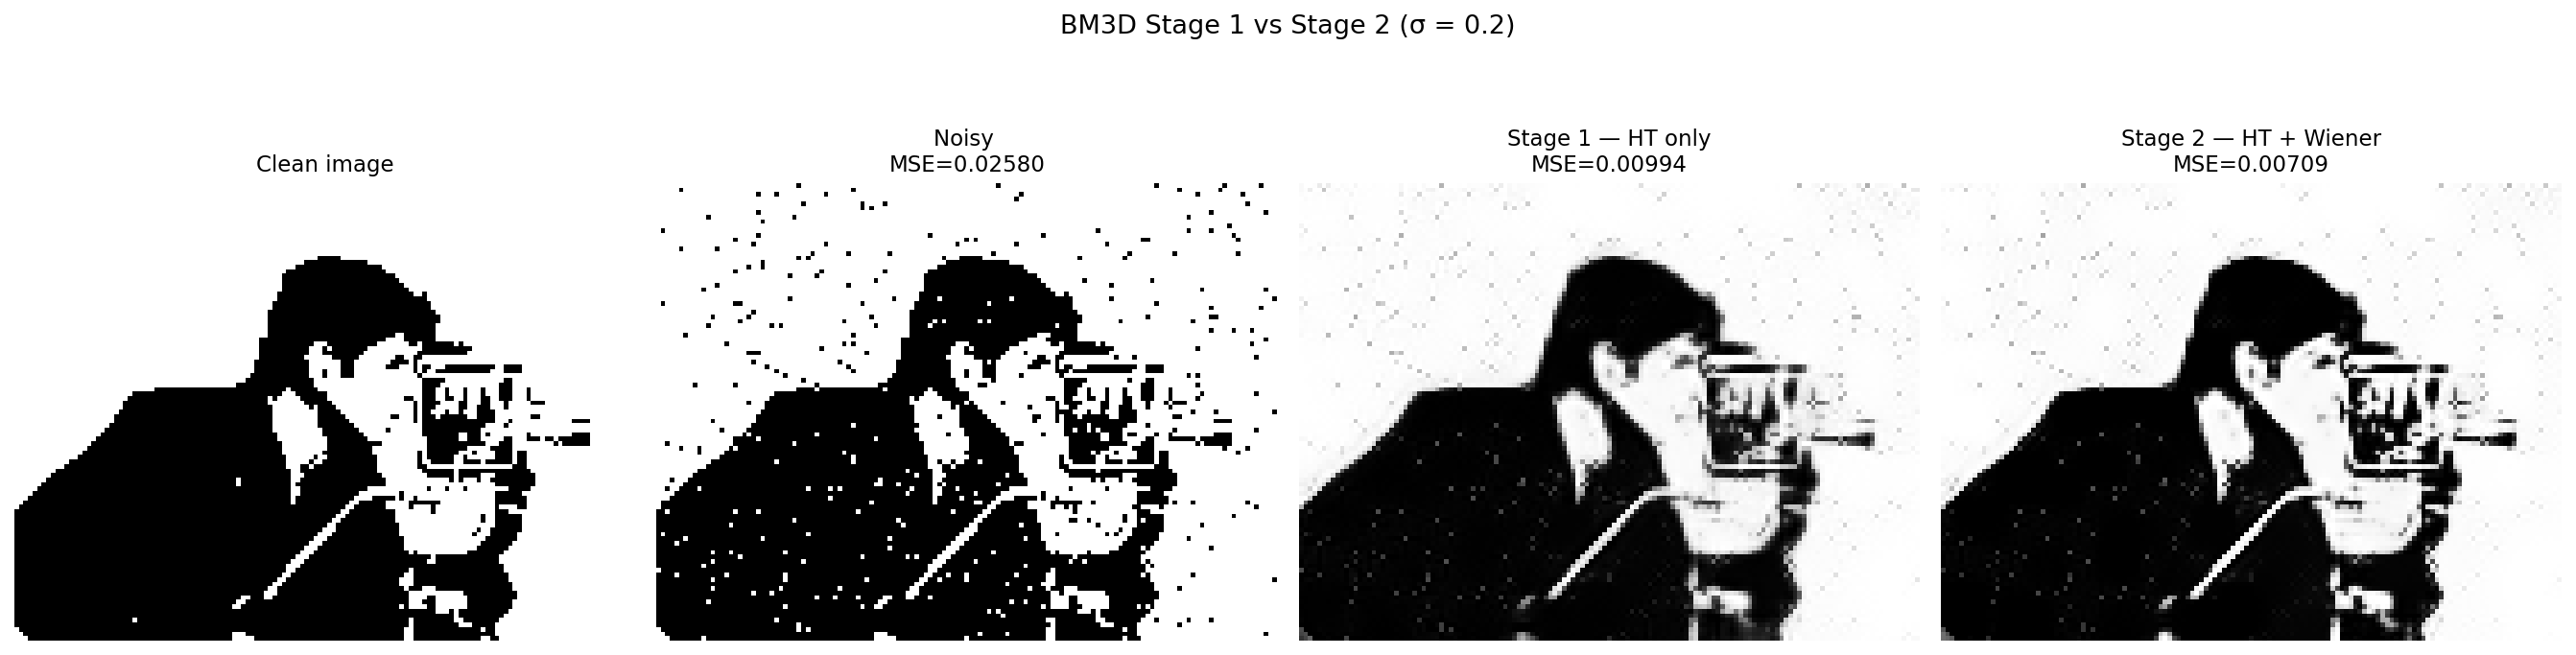
\includegraphics[width=\linewidth]{P01_1.png}
  \caption{Visual comparison of clean, noisy, Stage~1 (HT), and Stage~2 (Wiener) outputs. MSE values are shown in the sub-titles.}
\end{figure}

\end{solution}

\textbf{Subpart 2}
\begin{solution}

The assumed noise standard deviation $\sigma_Z$ (input to BM3D) was swept over the range $[0.05,\,1.0]$ in steps of $0.05$ (in $[0,1]$ image scale) and the output MSE against the clean image was recorded for each value.

\begin{figure}[H]
  \centering
  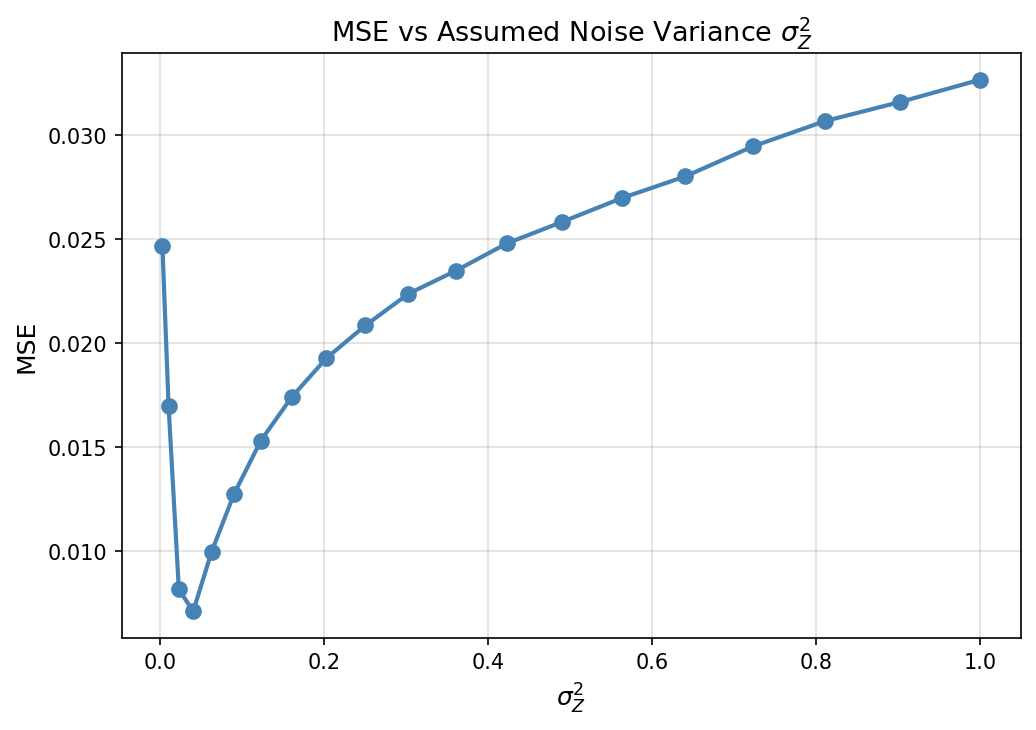
\includegraphics[width=0.65\linewidth]{P01_2.png}
  \caption{MSE vs.\ assumed noise variance $\sigma^2_Z$. The minimum MSE occurs near $\sigma_Z \approx 0.15$.}
\end{figure}

The curve exhibits a clear minimum around $\sigma^2_Z \approx 0.025$ (i.e.\ $\sigma_Z \approx 0.15$). That value is expected to be close to the original value of the sigma used to corrupt the image, that is why the curve hits a minimum at that point. Two regimes are visible:

\begin{itemize}
  \item \textbf{Under-denoising} ($\sigma_Z < \sigma_{\mathrm{true}}$): the threshold is too small, leaving residual noise in the output, so MSE remains elevated.
  \item \textbf{Over-denoising} ($\sigma_Z > \sigma_{\mathrm{true}}$): the threshold is too large, causing excessive smoothing and loss of detail. MSE increases monotonically and reaches its maximum at $\sigma_Z = 1.0$ (MSE $\approx 0.033$).
\end{itemize}

The curve is asymmetric: it rises steeply between the minimum and $\sigma_Z = 0.10$, but rises gradually for $\sigma_Z > 0.20$. When sigma is low, the threshold is low and the Wiener filtering coefficients have value near to 1, so not much noise is removed in that case. When sigma is high then erroneous grouping occurs. Wiener filtering in stage 2 can somehow compensate for erroneous but absolutely cannot compensate for the small groups.

\end{solution}

\textbf{Subpart 3}
\begin{solution}

To assess the contribution of the Wiener filter in Stage~2, it is replaced by a second pass of hard thresholding. Since the Stage~2 Wiener filter in the \texttt{bm3d} Python library is contained within the compiled \texttt{bm4d} binary (not modifiable), the following equivalent approach is adopted:

\begin{enumerate}
  \item Compute the basic estimate: $\hat{y}^{\mathrm{ht}} = \mathrm{BM3D}(z,\,\sigma;\;\mathrm{HARD\_THRESHOLDING})$.
  \item Apply a second HT pass on $\hat{y}^{\mathrm{ht}}$ with a reduced noise level $\sigma/2$ (reflecting the lower residual noise after Stage~1): $\hat{y}^{\mathrm{ht2}} = \mathrm{BM3D}(\hat{y}^{\mathrm{ht}},\,\sigma/2;\;\mathrm{HARD\_THRESHOLDING})$.
\end{enumerate}

This faithfully mimics Stage~2's structure (block-matching on a cleaner pilot image, then filtering) while substituting Wiener with HT. MSE results:

\begin{center}
\begin{tabular}{lc}
\toprule
Estimate & MSE \\
\midrule
Noisy input & 0.02580 \\
Stage 1 --- HT & 0.00994 \\
Stage 2 --- Wiener (standard BM3D) & 0.00709 \\
Stage 2 --- HT replacement & 0.01378 \\
\bottomrule
\end{tabular}
\end{center}

The Wiener-based Stage~2 achieves substantially lower MSE (0.00709) than the HT replacement (0.01850). The HT replacement is, in fact, \emph{worse} than even Stage~1 alone. This is because the reduced threshold $\sigma/2$ applied to an already partially denoised image over-smooths the output, and HT cannot adapt its shrinkage per-coefficient to the local signal energy. By contrast, Wiener shrinkage weights each coefficient by $|\hat{Y}^{\mathrm{ht}}_m|^2 / (|\hat{Y}^{\mathrm{ht}}_m|^2 + \sigma^2)$, which is close to~1 for dominant signal coefficients and close to~0 for noise-dominated ones — a behaviour impossible to replicate with a single global threshold. Visually, the image is over smoothed, no matter what the value of second sigma is taken the output remains over smooth. 

\begin{figure}[H]
  \centering
  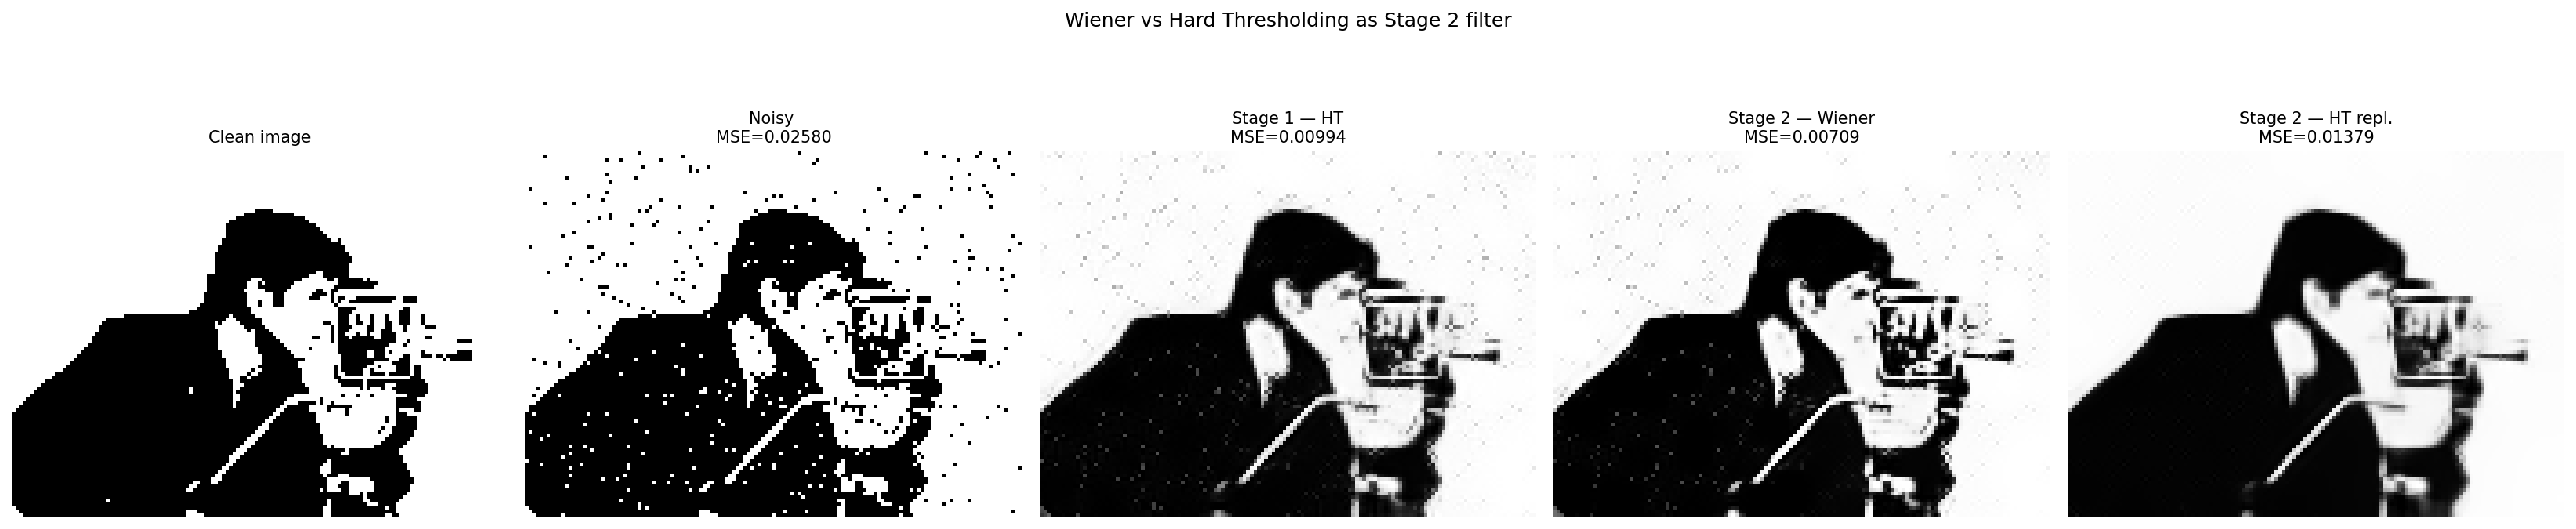
\includegraphics[width=\linewidth]{P01_3.png}
  \caption{Visual comparison of clean, noisy, Stage~1 (HT), Stage~2 (Wiener), and Stage~2 (HT replacement) outputs. MSE values are shown in the sub-titles.}
\end{figure}

\end{solution}

%----------------------------------------------------------------------
\questionheader{Problem 2: Zero Reference Deep Curve Estimation}
%----------------------------------------------------------------------

\begin{solution}

\subsection*{Hyperparameter Selection}

The Zero-DCE network enhances a low-light image $I$ by predicting a set of pixel-wise curve parameter maps $\mathcal{A} = \{A_n\}_{n=1}^{N}$ ($N=8$ in the paper) that iteratively adjust pixel intensities via the Light-Enhancement curve. The total training loss is:
\[
  \mathcal{L} = \mathcal{L}_{\mathrm{spa}} + \mathcal{L}_{\mathrm{exp}} + \mathcal{W}_{\mathrm{col}}\mathcal{L}_{\mathrm{col}} +\mathcal{W}_{\mathrm{tv,A}}\mathcal{L}_{\mathrm{tv,A}}
\]
where the four loss terms enforce spatial smoothness of $\mathcal{A}$, spatial consistency between enhanced and input images, color constancy (Grey-World hypothesis), and exposure control to a well-exposedness level $E$, respectively. For fine-tuning, the learning rate is reduced to $10^{-5}$ (one order below the original) to avoid catastrophic forgetting of the pre-trained weights. 

\subsection*{Results on VE-LOL-L Test Set}

The pre-trained Zero-DCE model and the per-image fine-tuned model were evaluated on five images from the VE-LOL-L dataset. PSNR and SSIM (with respect to the normal-light reference) are reported in Table~\ref{tab:p2_results}.

\begin{table}[H]
\centering
\caption{PSNR (dB) and SSIM for low-light input, pre-trained Zero-DCE, and fine-tuned Zero-DCE on five VE-LOL-L test images.}
\label{tab:p2_results}
\begin{tabular}{c ccc ccc cc}
\toprule
 & \multicolumn{2}{c}{Low-light input} & \multicolumn{2}{c}{Pre-trained} & \multicolumn{2}{c}{Fine-tuned} \\
\cmidrule(lr){2-3}\cmidrule(lr){4-5}\cmidrule(lr){6-7}
Image ID & PSNR & SSIM & PSNR & SSIM & PSNR & SSIM \\
\midrule
00698 & 8.29  & 0.0871 & 12.51 & 0.4134 & 17.46 & 0.4402 \\
00714 & 10.07 & 0.1712 & 19.48 & 0.8026 & 22.28 & 0.8168 \\
00743 & 10.48 & 0.3095 & 23.07 & 0.7931 & 24.01 & 0.7994 \\
00758 & 8.83  & 0.1354 & 15.92 & 0.5791 & 22.30 & 0.5487 \\
00781 & 8.63  & 0.1649 & 16.29 & 0.7594 & 18.67 & 0.7826 \\
\bottomrule
\end{tabular}
\end{table}

The only change made during fine-tuning relative to the original paper is the well-exposedness target $E$ in $\mathcal{L}_{\mathrm{exp}}$. The exposure loss penalises each local patch whose mean intensity deviates from $E$:
\[
  \mathcal{L}_{\mathrm{exp}} = \frac{1}{M}\sum_{k=1}^{M}\bigl|Y_k - E\bigr|,
\]
where $Y_k$ is the mean of the $k$-th non-overlapping patch of the enhanced image and $M$ is the total number of patches. The original paper fixes $E = 0.6$, which represents a well-exposed average scene. The VE-LOL-L test images, however, are significantly darker than the training distribution; their normal-light references have a lower mean intensity than a typical well-exposed photograph. Fine-tuning with a slightly reduced $E$ therefore steers the network towards an output mean that more closely matches the actual ground-truth illumination level of these specific images. The curve parameter maps $\mathcal{A}$ are updated on the single test image so that the exposure loss is minimised at the correct target, rather than at the over-bright $E = 0.6$ that was optimal for a generic training corpus. This image-specific adaptation of $E$ is the principal reason the fine-tuned outputs achieve better PSNR and SSIM than the pre-trained model on this dataset.

\begin{figure}[H]
  \centering
  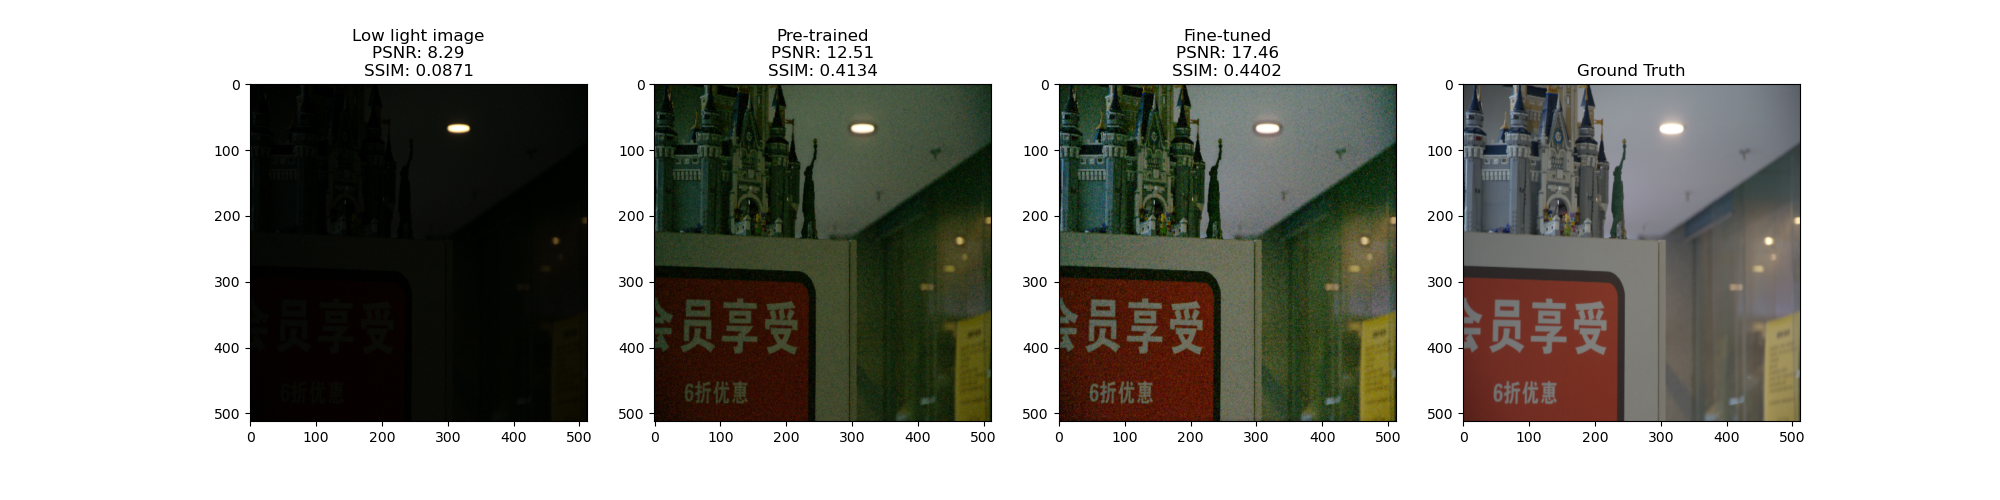
\includegraphics[width=\linewidth]{P02_00698.png}
  \caption{Image 00698: low-light input, pre-trained output, fine-tuned output, and ground truth.}
\end{figure}

\begin{figure}[H]
  \centering
  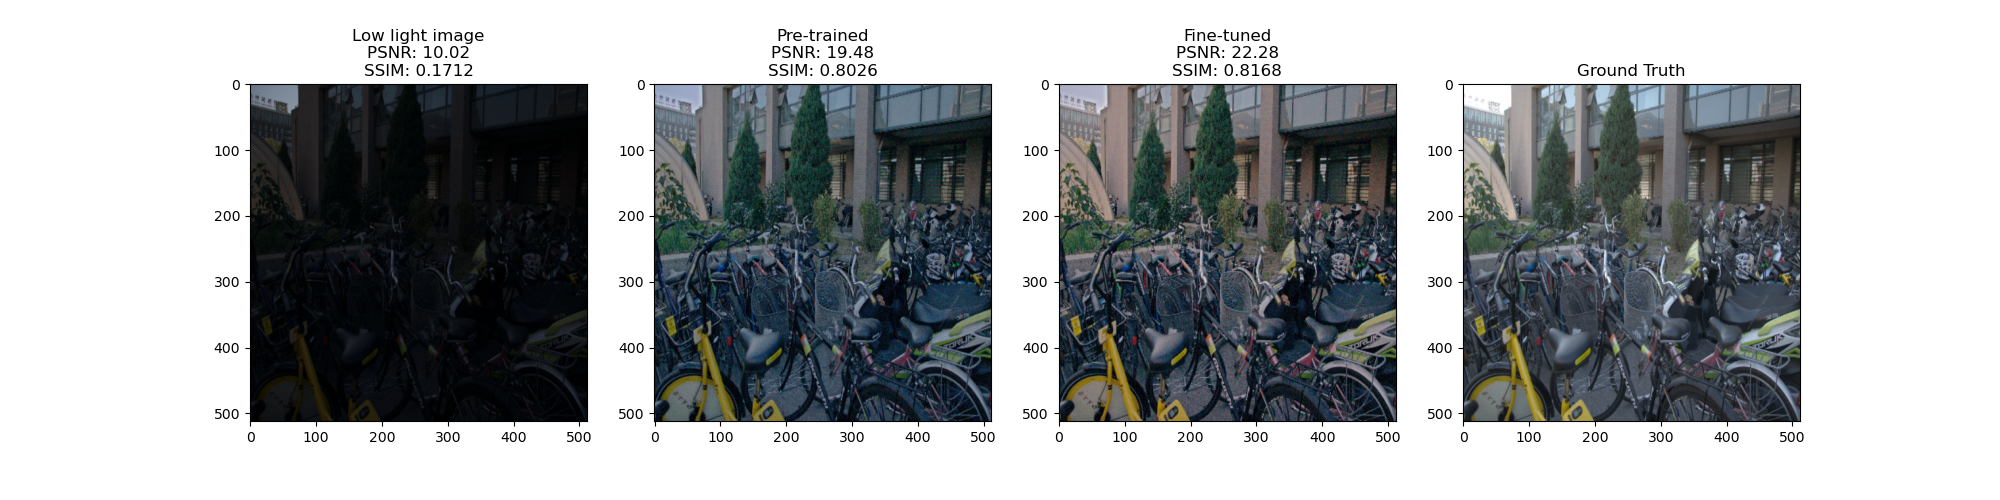
\includegraphics[width=\linewidth]{P02_00714.png}
  \caption{Image 00714: low-light input, pre-trained output, fine-tuned output, and ground truth.}
\end{figure}

\begin{figure}[H]
  \centering
  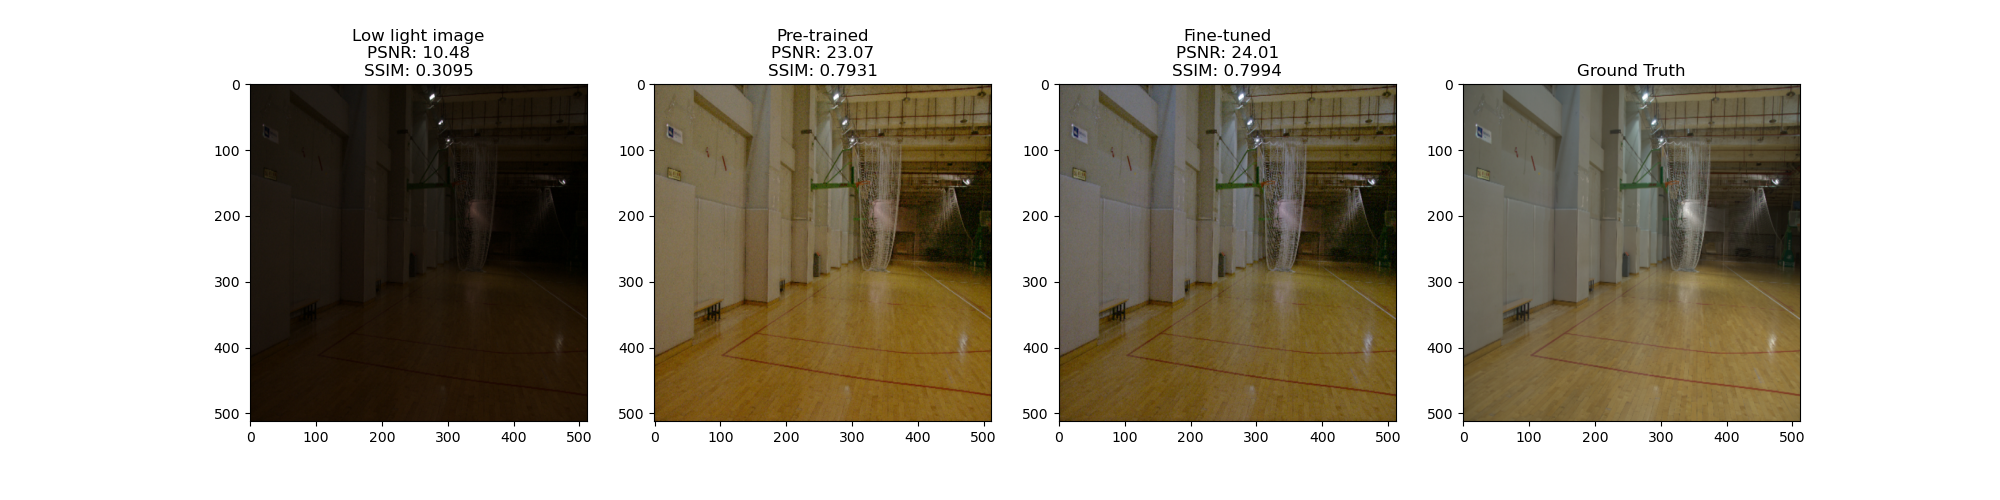
\includegraphics[width=\linewidth]{P02_00743.png}
  \caption{Image 00743: low-light input, pre-trained output, fine-tuned output, and ground truth.}
\end{figure}

\begin{figure}[H]
  \centering
  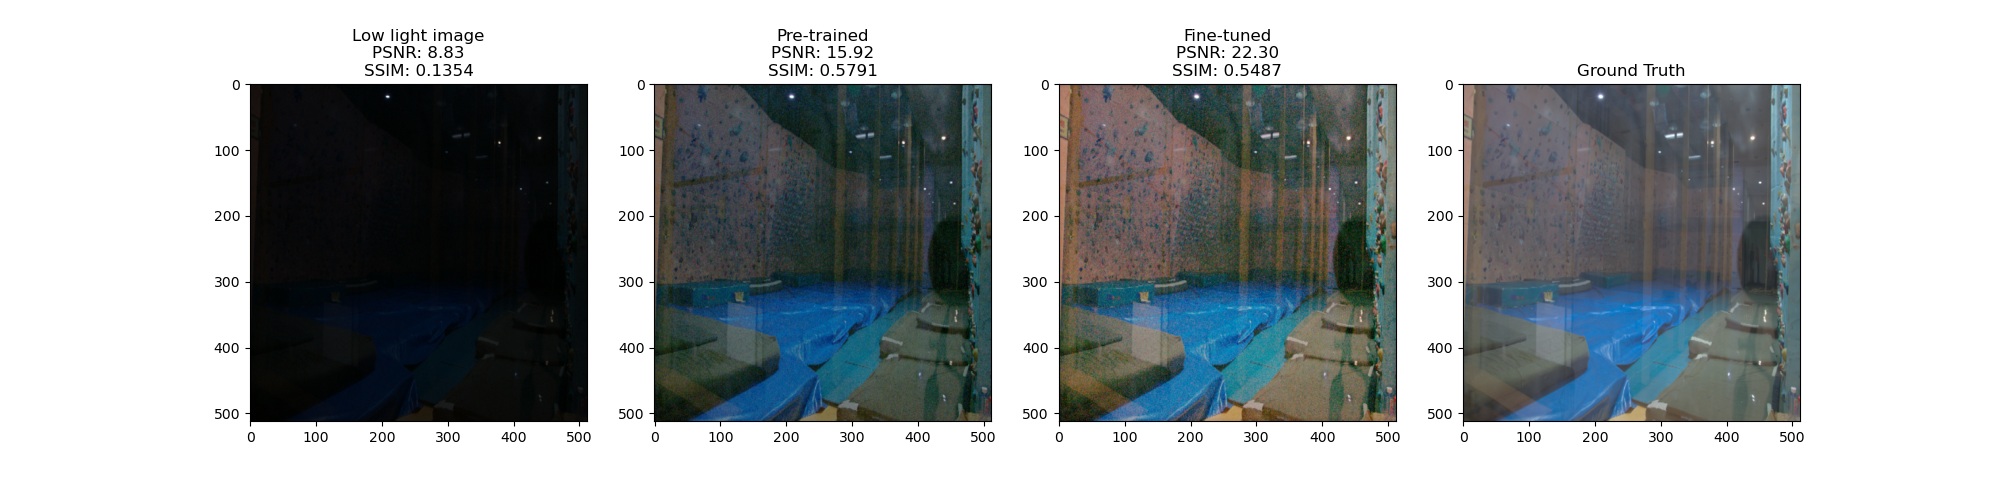
\includegraphics[width=\linewidth]{P02_00758.png}
  \caption{Image 00758: low-light input, pre-trained output, fine-tuned output, and ground truth.}
\end{figure}

\begin{figure}[H]
  \centering
  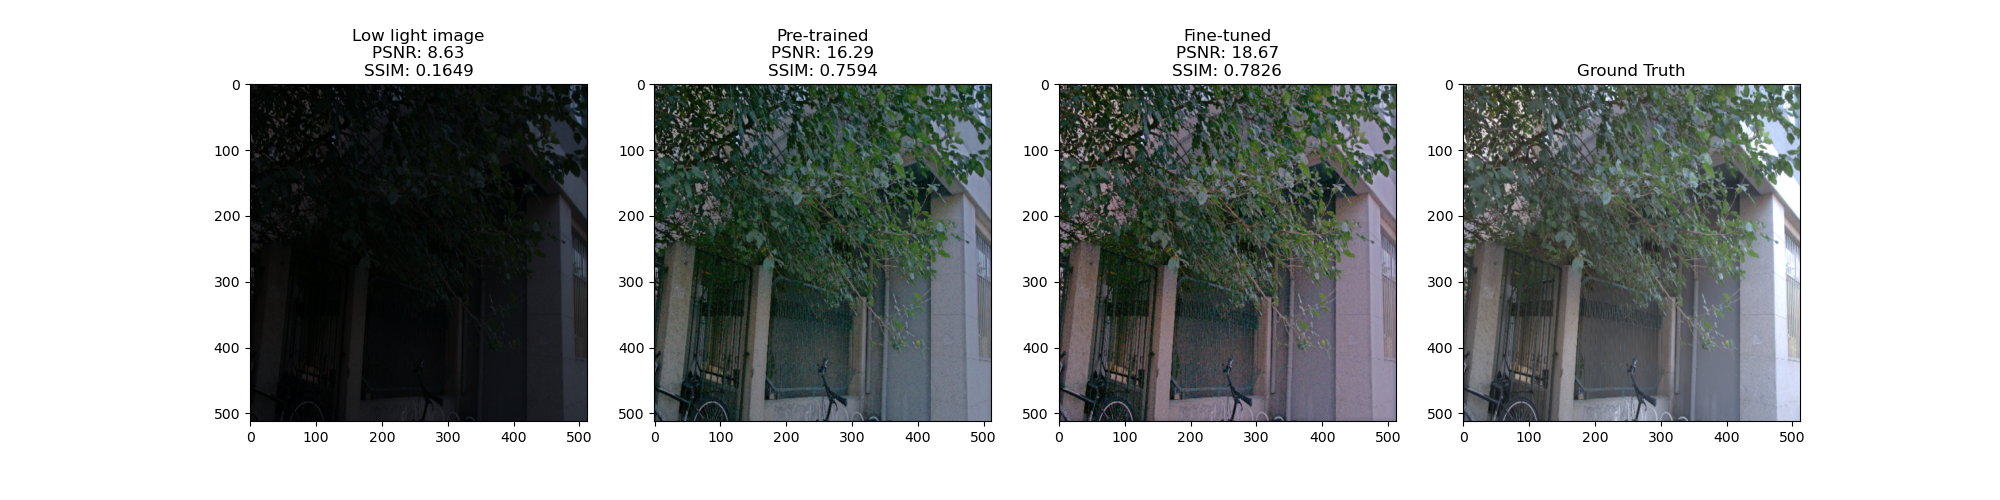
\includegraphics[width=\linewidth]{P02_00781.png}
  \caption{Image 00781: low-light input, pre-trained output, fine-tuned output, and ground truth.}
\end{figure}

\subsection*{Results on Own Low-Light Images}

Zero-DCE (pre-trained and fine-tuned) was also applied to four low-light photographs captured on a personal camera. Since no ground-truth reference is available, no quantitative metric is reported; results are shown qualitatively below.

\begin{figure}[H]
  \centering
  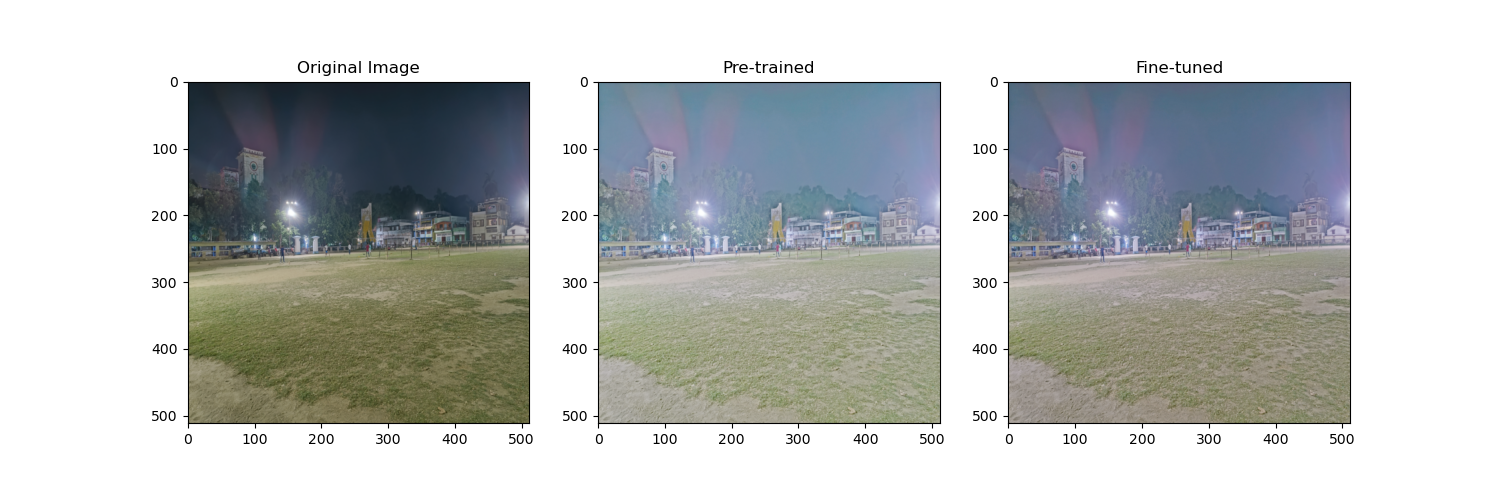
\includegraphics[width=\linewidth]{P02_IMG_1.jpg_own_camera.png}
  \caption{Own image 1 (football ground, night): original, pre-trained, and fine-tuned outputs.}
\end{figure}

\begin{figure}[H]
  \centering
  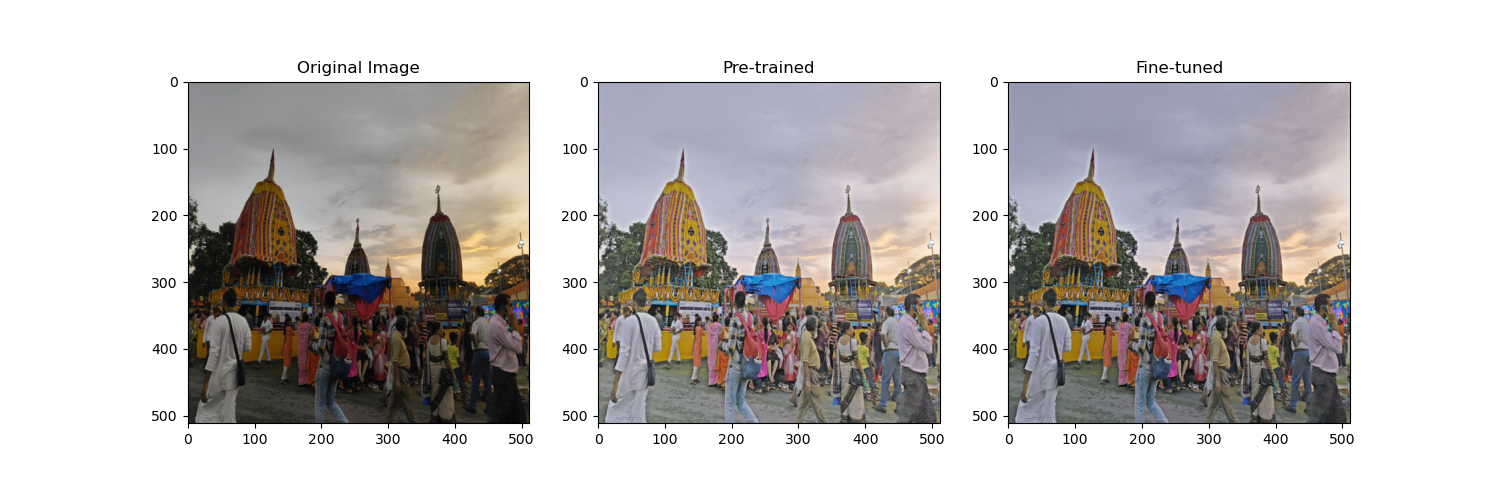
\includegraphics[width=\linewidth]{P02_IMG_2.jpg_own_camera.png}
  \caption{Own image 2 (temple, dusk): original, pre-trained, and fine-tuned outputs.}
\end{figure}

\begin{figure}[H]
  \centering
  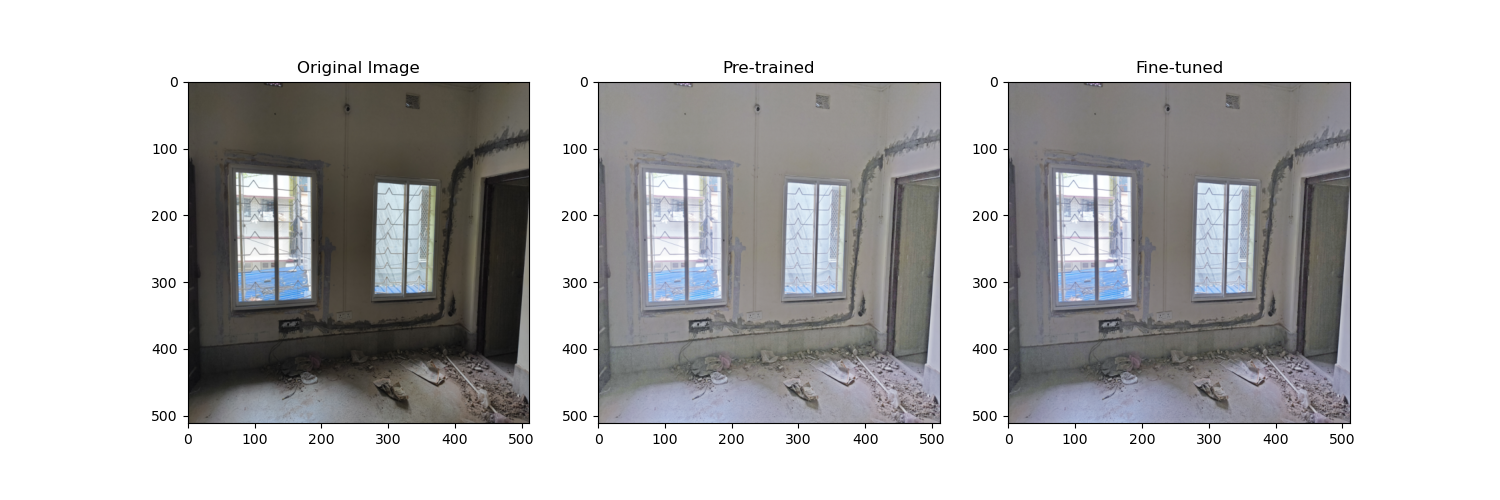
\includegraphics[width=\linewidth]{P02_IMG_3.jpg_own_camera.png}
  \caption{Own image 3 (indoor, low light): original, pre-trained, and fine-tuned outputs.}
\end{figure}

\begin{figure}[H]
  \centering
  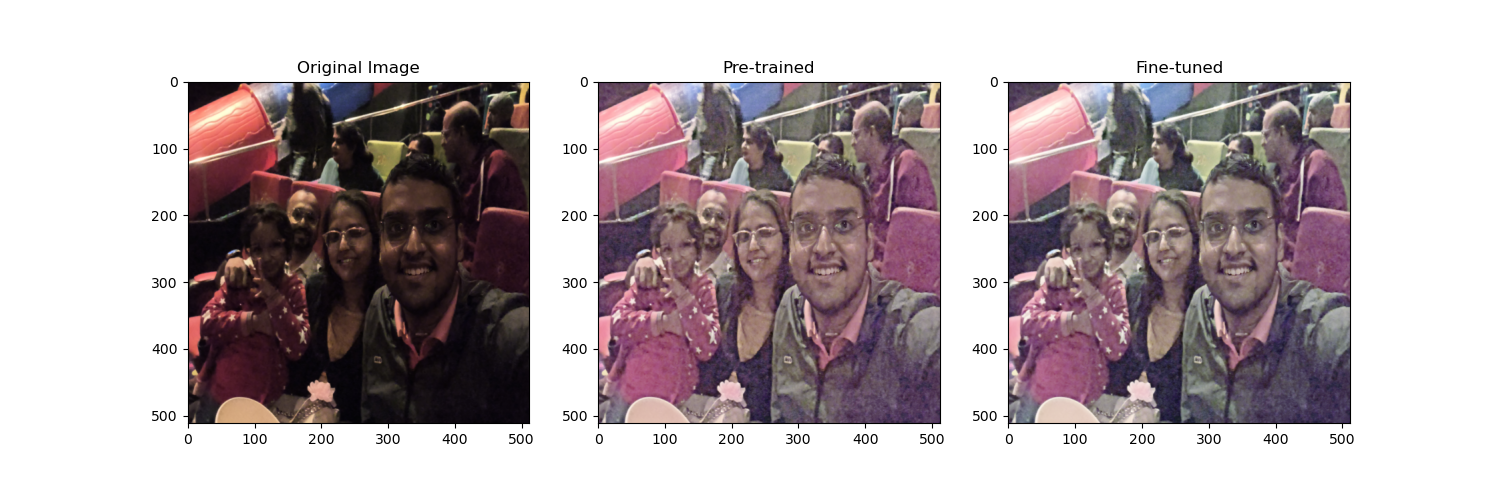
\includegraphics[width=\linewidth]{P02_IMG_4.jpg_own_camera.png}
  \caption{Own image 4 (group photo, dim light): original, pre-trained, and fine-tuned outputs.}
\end{figure}

For all four personal images, the pre-trained model fits well. While the fine tuned model gives slight improvements. 
\end{solution}

\end{document}
